%%\documentclass[a4paper,12pt,oneside]{llncs}
\documentclass[12pt,letterpaper]{article}
\usepackage[right=2cm,left=3cm,top=2cm,bottom=2cm,headsep=0cm]{geometry}

%%%%%%%%%%%%%%%%%%%%%%%%%%%%%%%%%%%%%%%%%%%%%%%%%%%%%%%%%%%
%% Juego de caracteres usado en el archivo fuente: UTF-8
\usepackage{ucs}
\usepackage[utf8x]{inputenc}

%%%%%%%%%%%%%%%%%%%%%%%%%%%%%%%%%%%%%%%%%%%%%%%%%%%%%%%%%%%
%% Juego de caracteres usado en la salida dvi
%% Otra posibilidad: \usepackage{t1enc}
\usepackage[T1]{fontenc}

%%%%%%%%%%%%%%%%%%%%%%%%%%%%%%%%%%%%%%%%%%%%%%%%%%%%%%%%%%%
%% Ajusta maergenes para a4
%\usepackage{a4wide}

%%%%%%%%%%%%%%%%%%%%%%%%%%%%%%%%%%%%%%%%%%%%%%%%%%%%%%%%%%%
%% Uso fuente postscript times, para que los ps y pdf queden y pequeños...
\usepackage{times}

%%%%%%%%%%%%%%%%%%%%%%%%%%%%%%%%%%%%%%%%%%%%%%%%%%%%%%%%%%%
%% Posibilidad de hipertexto (especialmente en pdf)
%\usepackage{hyperref}
\usepackage[bookmarks = true, colorlinks=true, linkcolor = black, citecolor = black, menucolor = black, urlcolor = black]{hyperref}

%%%%%%%%%%%%%%%%%%%%%%%%%%%%%%%%%%%%%%%%%%%%%%%%%%%%%%%%%%%
%% Graficos 
\usepackage{graphics,graphicx}

%%%%%%%%%%%%%%%%%%%%%%%%%%%%%%%%%%%%%%%%%%%%%%%%%%%%%%%%%%%
%% Ciertos caracteres "raros"...
\usepackage{latexsym}

%%%%%%%%%%%%%%%%%%%%%%%%%%%%%%%%%%%%%%%%%%%%%%%%%%%%%%%%%%%
%% Matematicas aun más fuertes (american math dociety)
\usepackage{amsmath}

%%%%%%%%%%%%%%%%%%%%%%%%%%%%%%%%%%%%%%%%%%%%%%%%%%%%%%%%%%%
\usepackage{multirow} % para las tablas
\usepackage[spanish,es-tabla]{babel}

%%%%%%%%%%%%%%%%%%%%%%%%%%%%%%%%%%%%%%%%%%%%%%%%%%%%%%%%%%%
%% Fuentes matematicas lo mas compatibles posibles con postscript (times)
%% (Esto no funciona para todos los simbolos pero reduce mucho el tamaño del
%% pdf si hay muchas matamaticas....
\usepackage{mathptm}

%%% VARIOS:
%\usepackage{slashbox}
\usepackage{verbatim}
\usepackage{array}
\usepackage{listings}
\usepackage{multirow}

%% MARCA DE AGUA
%% Este package de "draft copy" NO funciona con pdflatex
%%\usepackage{draftcopy}
%% Este package de "draft copy" SI funciona con pdflatex
%%%\usepackage{pdfdraftcopy}
%%%%%%%%%%%%%%%%%%%%%%%%%%%%%%%%%%%%%%%%%%%%%%%%%%%%%%%%%%%
%% Indenteacion en español...
\usepackage[spanish]{babel}

\usepackage{listings}
% Para escribir código en C
% \begin{lstlisting}[language=C]
% #include <stdio.h>
% int main(int argc, char* argv[]) {
% puts("Hola mundo!");
% }
% \end{lstlisting}


\title{Práctica 0}
\author{Jesús Rodríguez Heras\\
	Arantzazu Otal Alberro}

\begin{document}
	
	\maketitle
%	\begin{abstract} %Poner esto en todas las prácticas de PCTR
%%		\begin{center}
%%			\noindent
%			
%%		\end{center}
%	\end{abstract}
	\thispagestyle{empty}
	\newpage
	
%	\tableofcontents
%	\newpage
	
	%%\listoftables
	%%\newpage
	
	%%\listoffigures
	%%\newpage
	
	%%%% REAL WORK BEGINS HERE:
	
	%%Configuracion del paquete listings
	\lstset{language=bash, numbers=left, numberstyle=\tiny, numbersep=10pt, firstnumber=1, stepnumber=1, basicstyle=\small\ttfamily, tabsize=1, extendedchars=true, inputencoding=latin1}
	
Para la instalación de vagrant necesitamos git y virtualbox:
\begin{itemize}
	\item \texttt{apt-get install git}
	\item \texttt{apt-get install virtualbox}
\end{itemize}
Una vez instalados, toca instalar vagrant con \texttt{apt-get install vagrant}.

A continuación, usamos el comando \texttt{vagrant init hashicorp/precise64} para descargar la máquina ``precise64'' de las disponibles en hashicorp.

También tendremos que crear un pequeño script para que nos instale apache llamado \texttt{bootstrap.sh}.
\begin{lstlisting}[language=Bash]
#!/usr/bin/env bash

apt-get update
apt-get install -y apache2
if ! [ -L /var/www ]; then
    rm -rf /var/www
    ln -fs /vagrant /var/www
fi
\end{lstlisting}

Antes de lanzar la máquina, tendremos que editar el archivo de configuración de vagrant (\texttt{Vagrantfile}) dejándolo de la siguiente forma:
\begin{lstlisting}[language=Bash]
Vagrant.configure("2") do |config|
    config.vm.box = "hashicorp/precise64"
    config.vm.provision :shell, path: "bootstrap.sh"
    config.vm.network :forwarded_port, guest: 80, host: 4567
end
\end{lstlisting}

Para lanzar la máquina virtual usamos \texttt{vagrant up} y podremos ver que en consola aparece lo siguiente:
\begin{figure}[h]
	\centering
	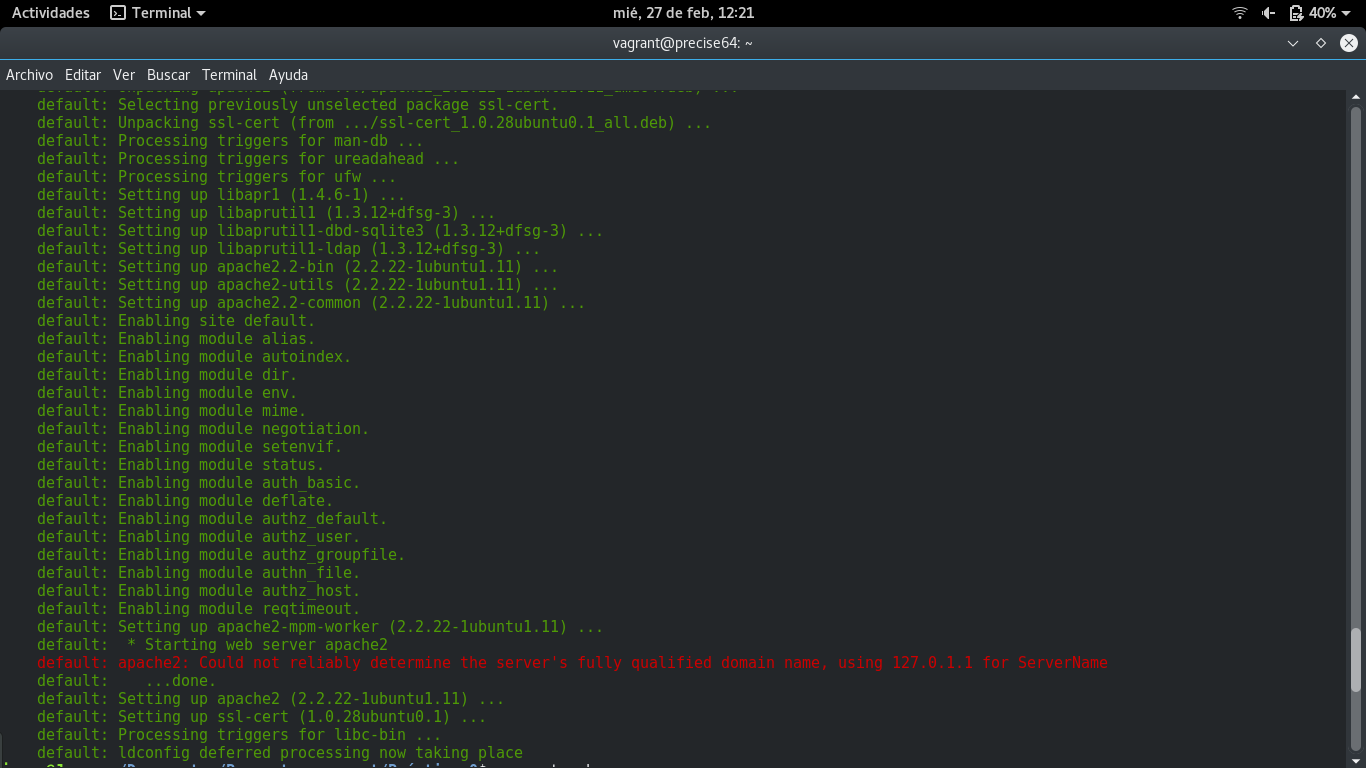
\includegraphics[scale=0.3]{Instalacion.png}
\end{figure}
\newpage
Cuando se ha lanzado, accedemos a ella a través de ssh mediante el comando \texttt{vagrant ssh} y probamos que el servidor de apache esté ejecutándose con \texttt{wget -qO- 127.0.0.1}.
\begin{figure}[h]
	\centering
	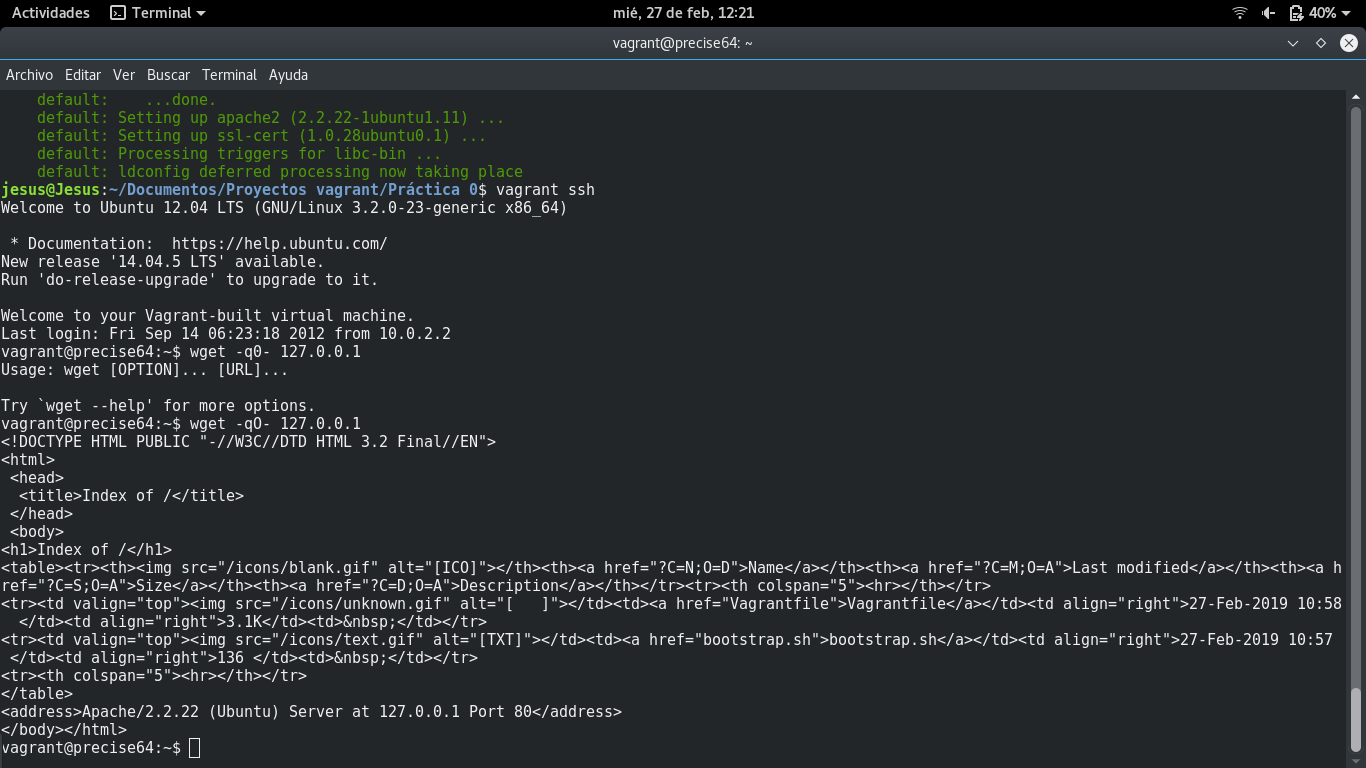
\includegraphics[scale=0.3]{ssh.png}
\end{figure}

Para comprobar que todo funciona correctamente entramos en la dirección \texttt{127.0.0.1:4567} desde el navegador de nuestro ordenador y podremos ver la carpeta compartida desde el navegador.
\begin{figure}[h]
	\centering
	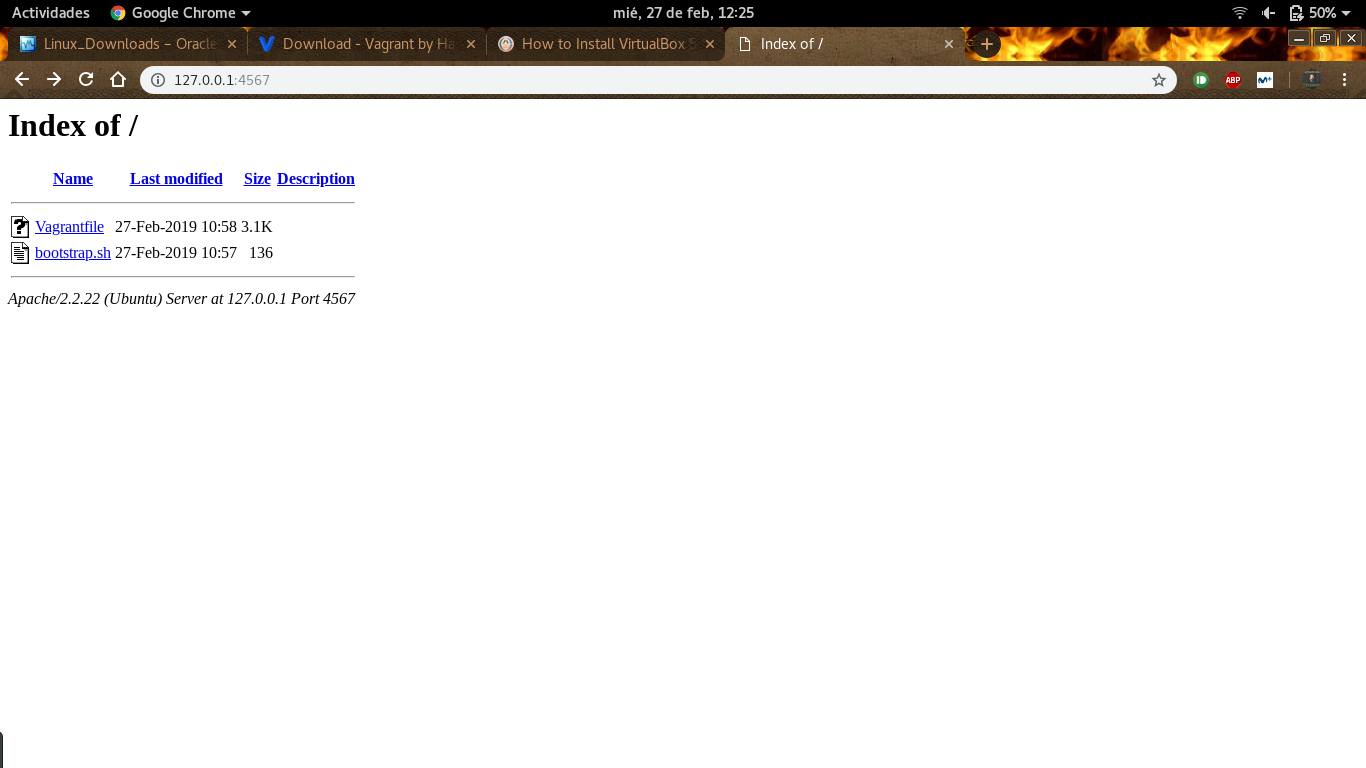
\includegraphics[scale=0.3]{Carpeta1.png}
\end{figure}
\newpage
Si hacemos cambios en la carpeta compartida y actualizamos el navegador, podremos ver los cambios realizados.
\begin{figure}[h]
	\centering
	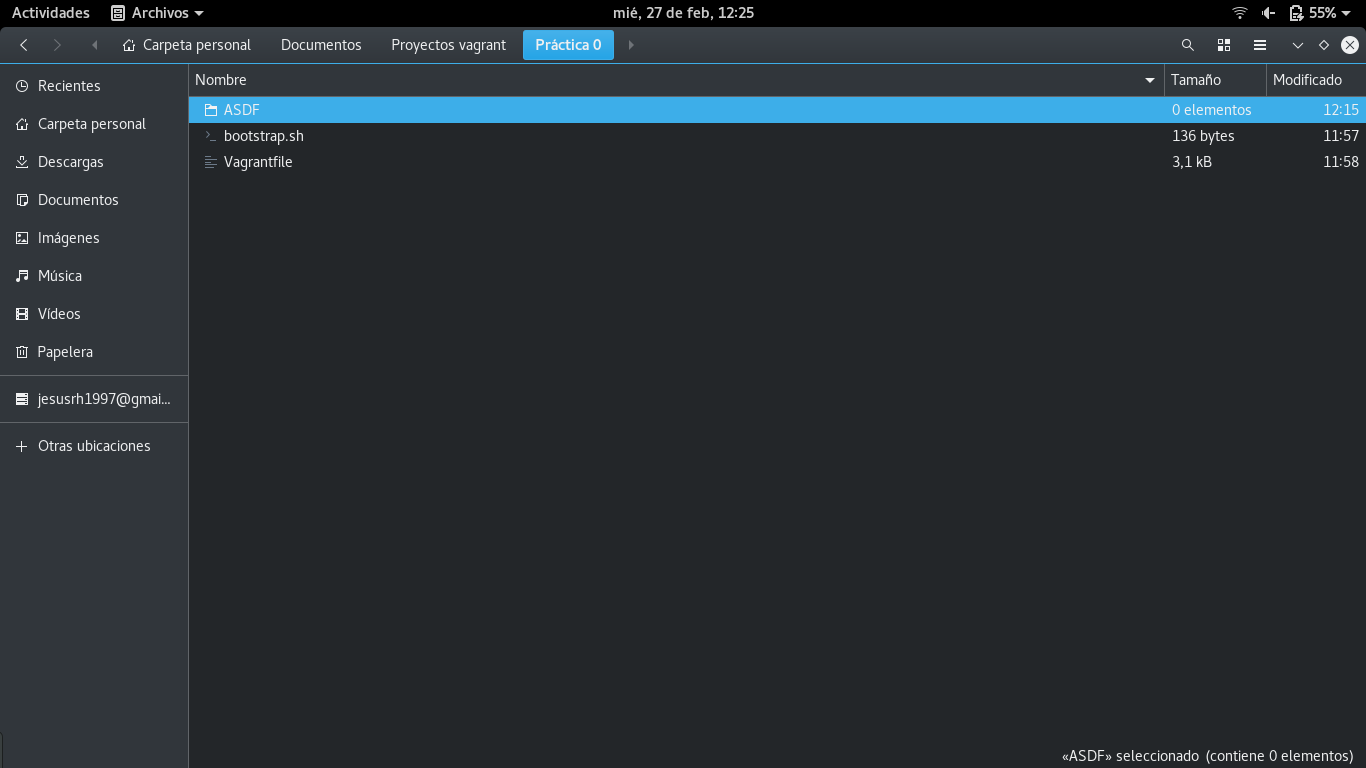
\includegraphics[scale=0.3]{Carpeta2.png}
\end{figure}
\begin{figure}[h]
	\centering
	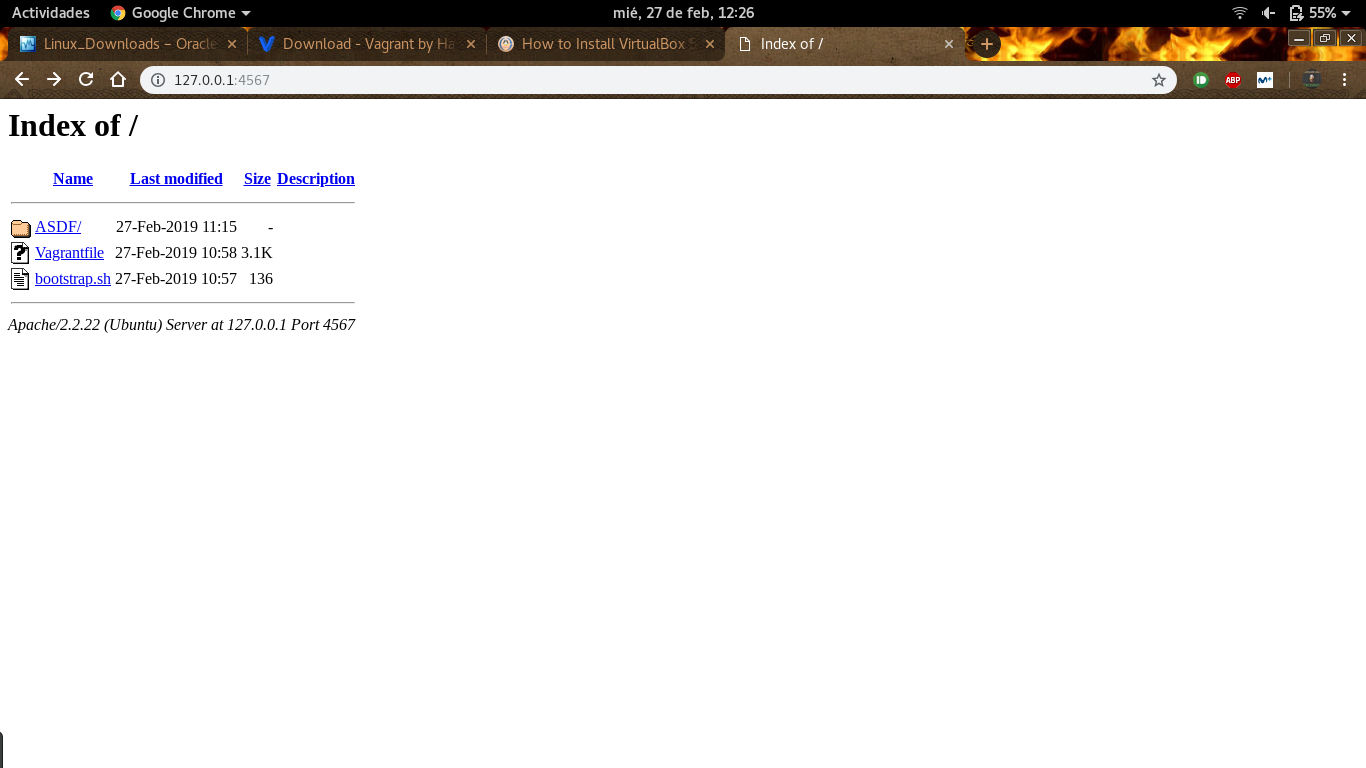
\includegraphics[scale=0.3]{Carpeta3.png}
\end{figure}

\end{document}